\lstset{backgroundcolor = \color{lightgray},
  basicstyle=\ttfamily,
  keywordstyle=\color{blue}\ttfamily,
  stringstyle=\color{red}\ttfamily,
  commentstyle=\color{green}\ttfamily,
  language = Matlab
}

\section{Annotated code}

The Matlab code here is taken from the website: \url{http://cvlab.epfl.ch/software/daisy}.

\subsection{Compute histograms for each pixel}

\begin{lstlisting}
lollero
\end{lstlisting}

\subsection{Normalize histograms to unit norm}

\subsection{DAISY descriptor is computed}

\section{Directional derivative images}

\begin{figure}\label{fig:face}
  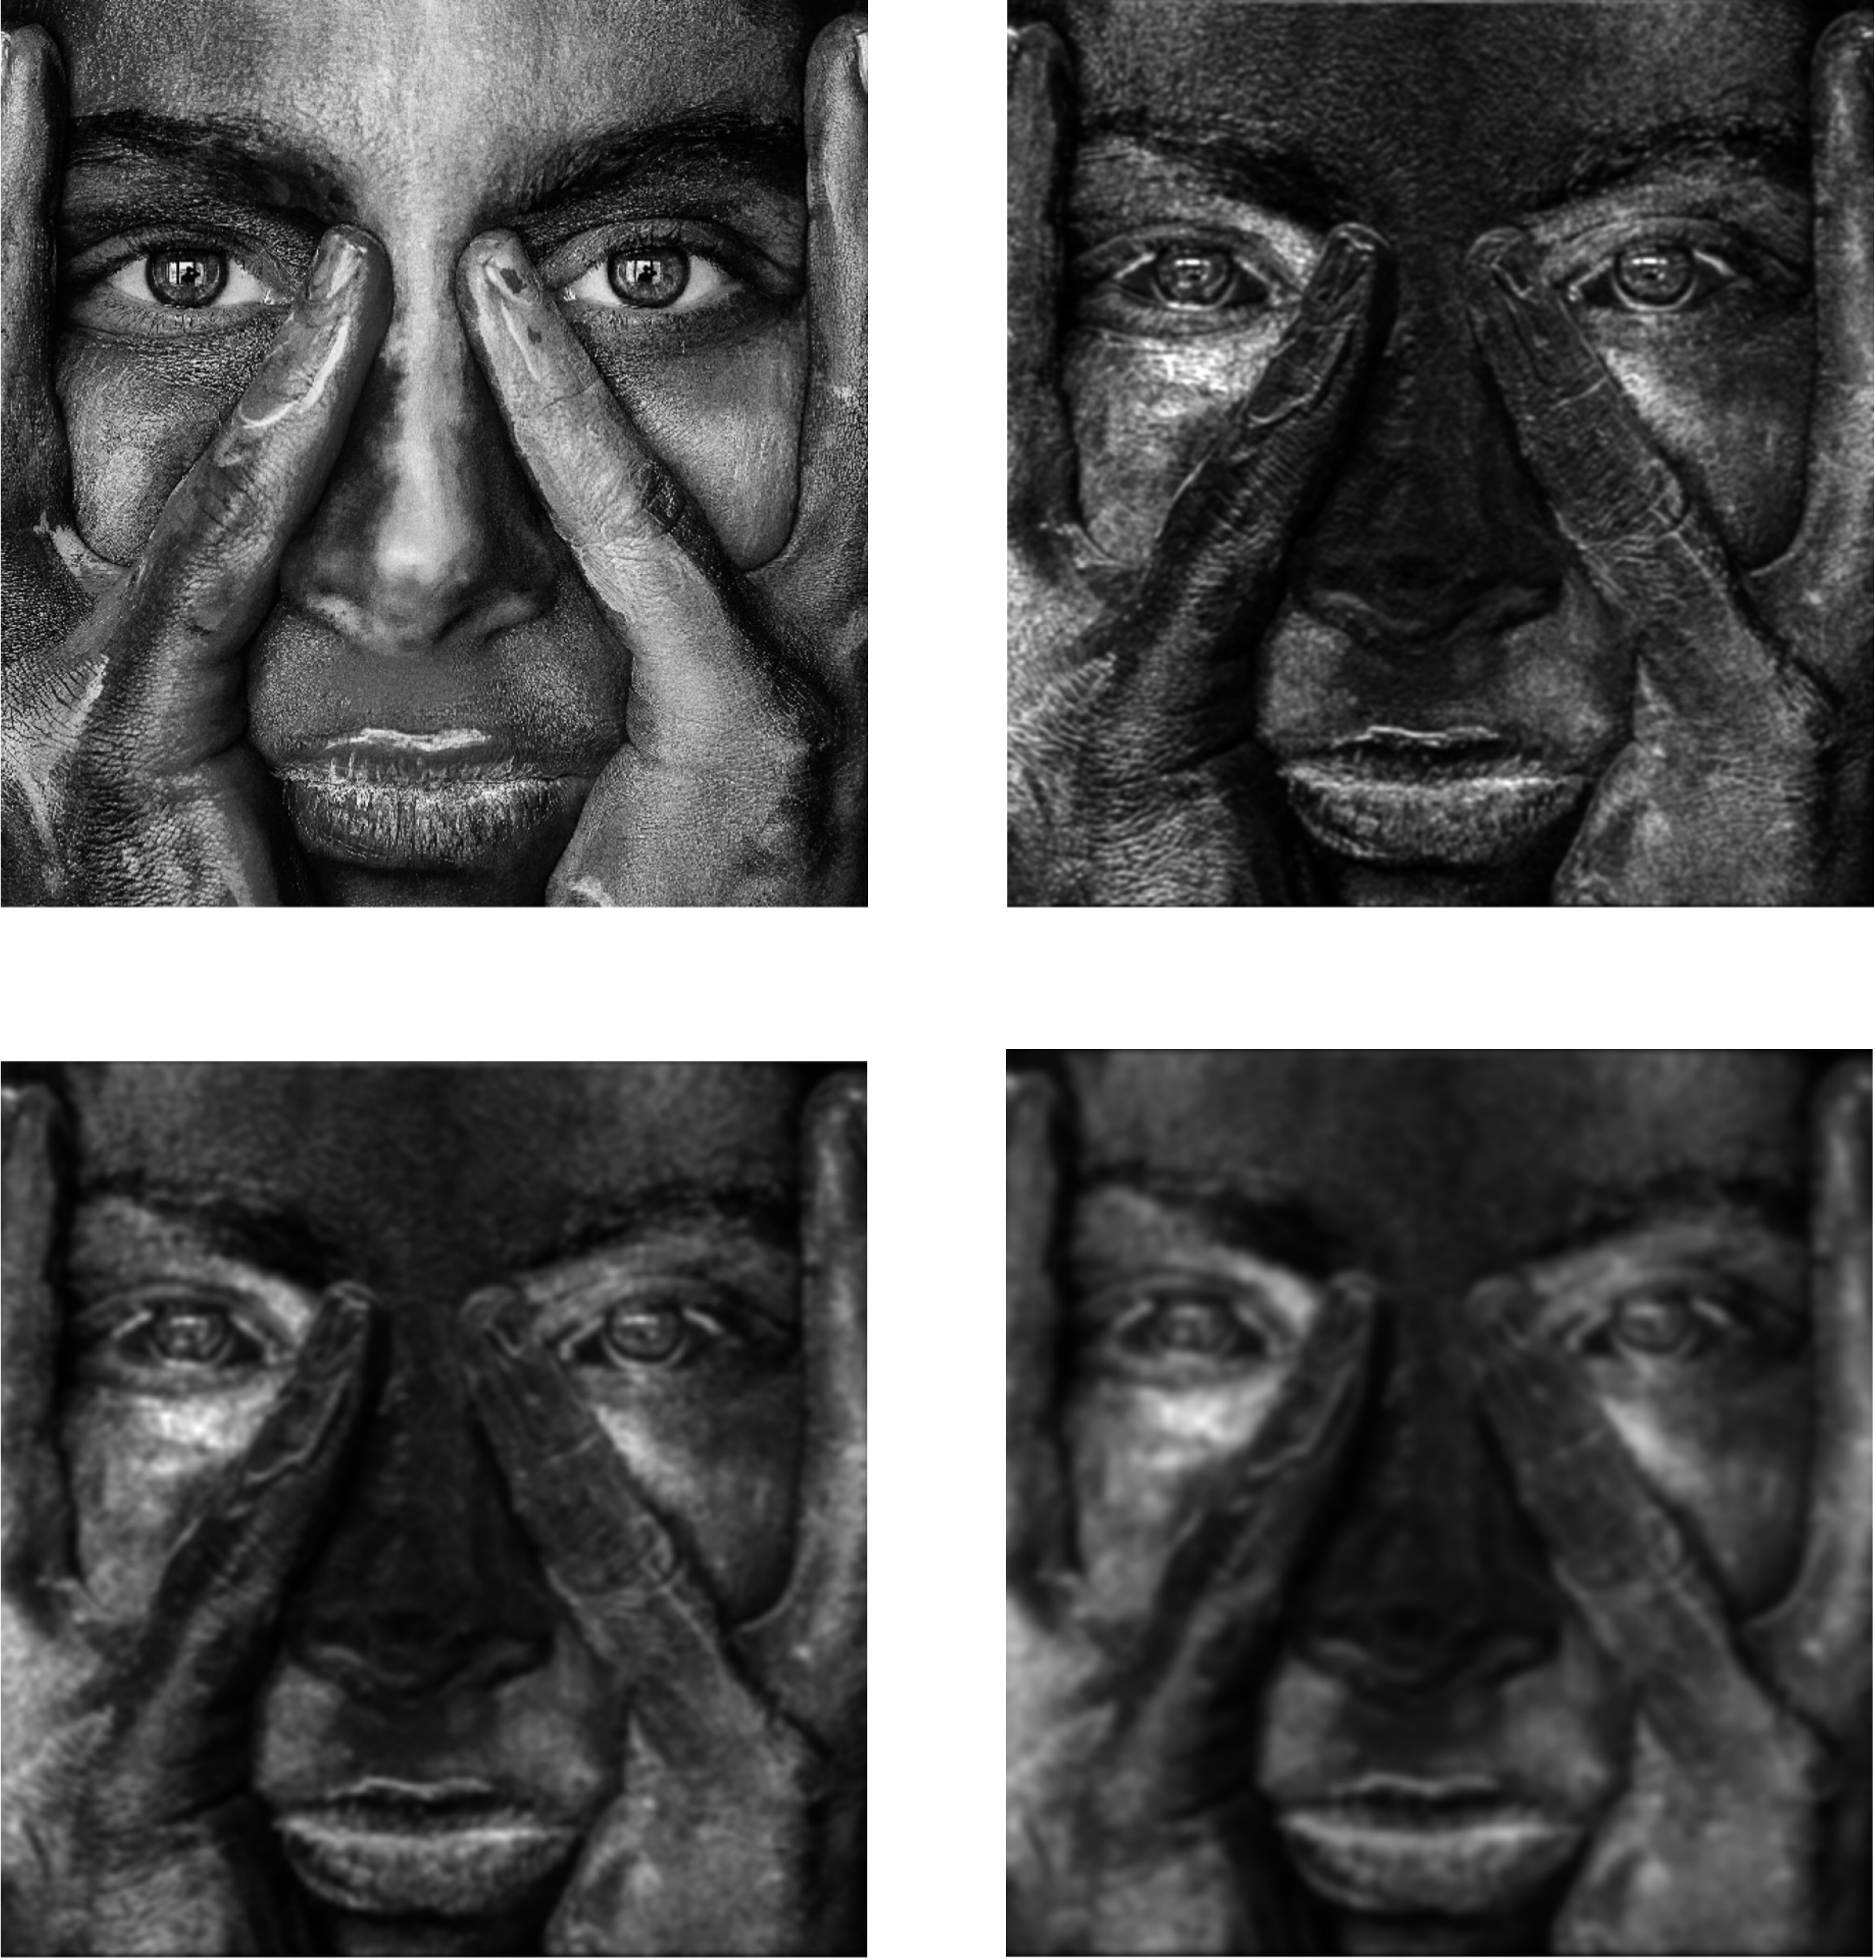
\includegraphics[width=\textwidth]{image1-table}
  \caption{Three directional derivative images and the original in the top-left
  corner}
\end{figure}

\begin{figure}\label{fig:grasshopper}
  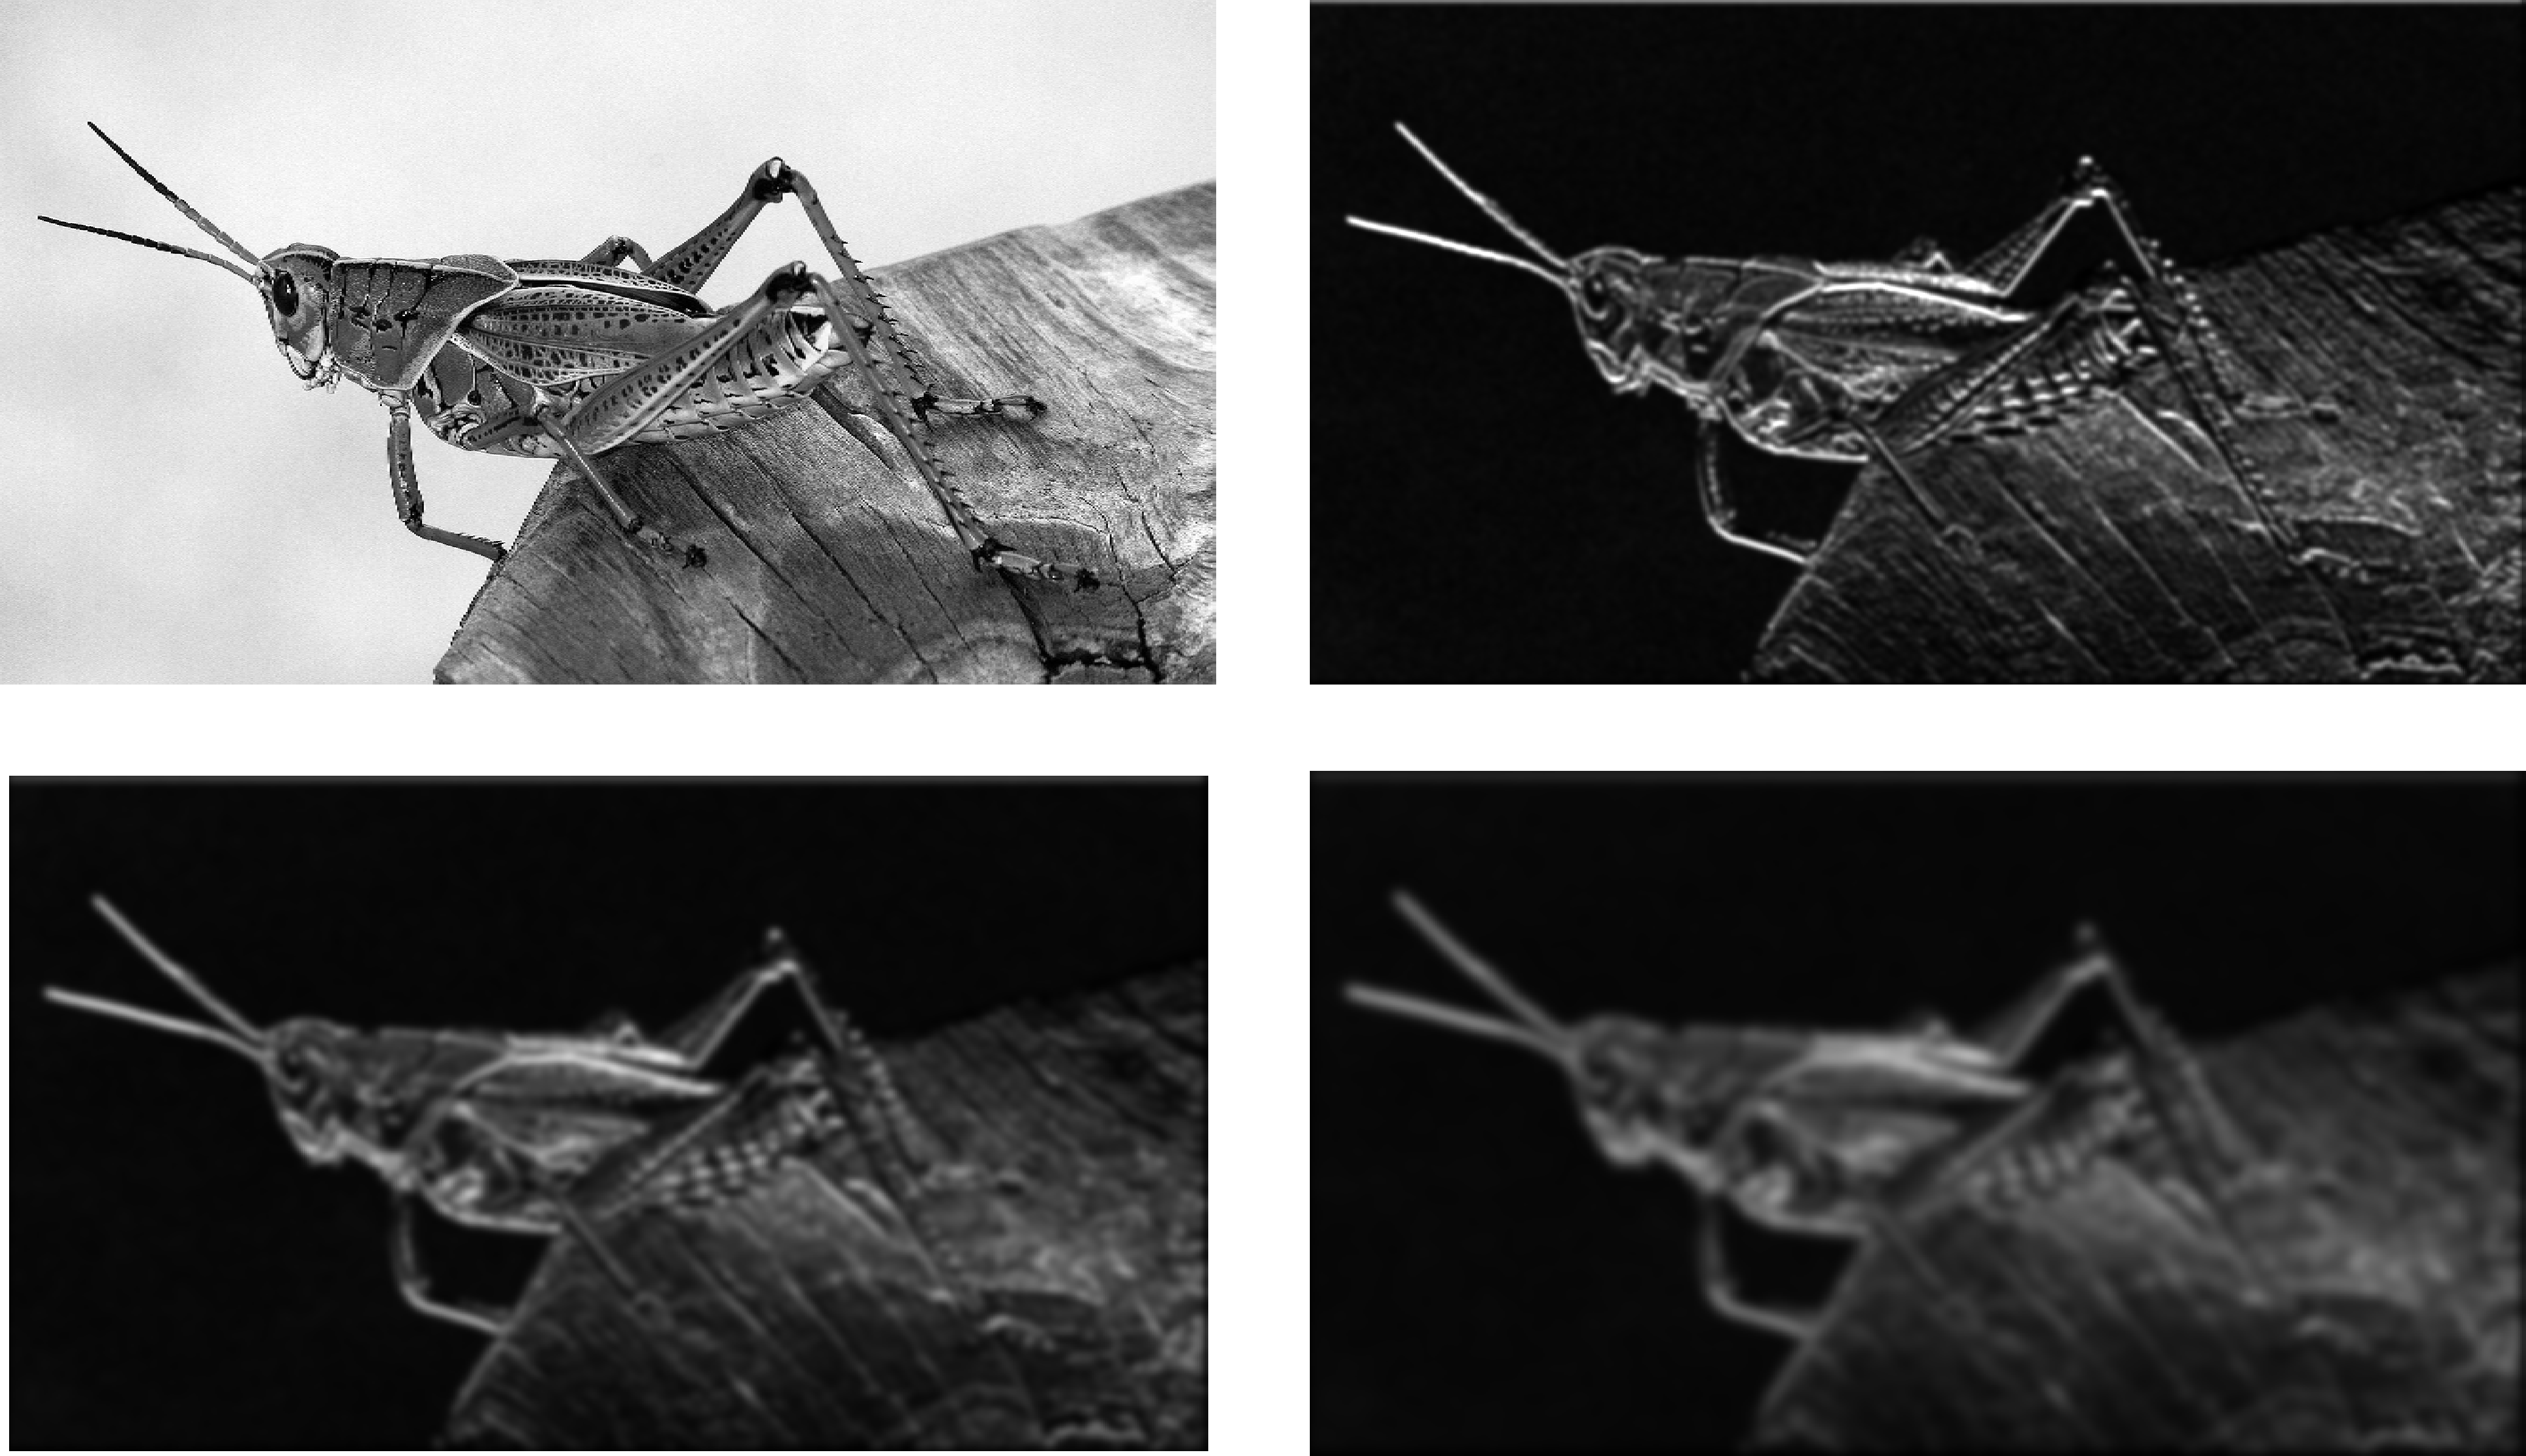
\includegraphics[width=\textwidth]{image2-table}
  \caption{Three directional derivative images and the original in the top-left
  corner}
\end{figure}

\section{Description of feature points}
